\documentclass[tikz,border=12pt]{standalone}
\usepackage[T1]{fontenc}
\usepackage{tgheros}
\usepackage{sfmath}
\usepackage{amsmath}
\usepackage{fontawesome5}
\usepackage{tikz}
\usetikzlibrary{arrows.meta,positioning,shapes.geometric,fit,backgrounds,calc}
\usepackage{xcolor}

\renewcommand{\familydefault}{\sfdefault}

% Harvard Crimson & ETH Zurich Academic Semantic Palette
\definecolor{harvardcrimson}{HTML}{A51C30}
\definecolor{ethdarkblue}{HTML}{1F407A}
\definecolor{ethblue}{HTML}{215CAF}
\definecolor{ethpetrol}{HTML}{007A87}
\definecolor{ethbronze}{HTML}{B87333}
\definecolor{ethslate}{HTML}{475569}
\definecolor{cardbg}{HTML}{F8FAFC}
\definecolor{cardborder}{HTML}{CBD5E1}
\definecolor{safeTeal}{HTML}{10B981}
\definecolor{amberWarn}{HTML}{D97706}

\begin{document}
\begin{tikzpicture}[
  font=\sffamily,
  >=Stealth,
  scale=1.0
]

  % ---------------------------------------------------------------------------
  % TOP HEADER CARD
  % ---------------------------------------------------------------------------
  \node[draw=ethdarkblue, fill=ethdarkblue!5, rounded corners=6pt, line width=1.1pt, text width=9.20in, inner sep=8pt, align=center] (title) at (4.60in, 0) {
    {\normalsize\bfseries\color{ethdarkblue}\faIcon{ruler-horizontal}\;\; DYNAMIC STOPPING DISTANCE: SENSE-TO-ACTUATION DELAY AS PHYSICAL DISPLACEMENT}\\[3pt]
    {\scriptsize\color{ethslate}Translating Milliseconds of Computational Latency into Physical Centimeters of Unguided Collision Hazard}
  };

  % Equation Box
  \node[draw=cardborder, fill=cardbg, rounded corners=5pt, line width=0.9pt, text width=9.20in, inner sep=7pt, align=center, below=0.12in of title] (eq) {
    {\small $\displaystyle d_{\text{stop}}(v_0, \Delta t_{\text{delay}}) \;=\; \underbrace{v_0 \cdot \Delta t_{\text{delay}}}_{\substack{\text{\textbf{\color{ethblue}Phase 1: Linear Reaction Travel}}\\\text{\scriptsize\color{ethslate}(Coasting during computational delay)}}} \;+\; \underbrace{\frac{v_0^2}{2 a_{\text{max}}}}_{\substack{\text{\textbf{\color{ethbronze}Phase 2: Quadratic Braking Distance}}\\\text{\scriptsize\color{ethslate}(Mechanical deceleration to rest)}}}$}
  };

  % ---------------------------------------------------------------------------
  % COORDINATE MAPPING: 1 meter = 16.0 inches (1 cm = 0.16 in)
  % Origin at 0.60in from left, spanning to 0.50m (8.00in)
  % ---------------------------------------------------------------------------
  \coordinate (X0) at (0.60in, -1.50in);
  
  % ---------------------------------------------------------------------------
  % ROW 1: NOMINAL EXECUTION (P50 = 30 ms)
  % ---------------------------------------------------------------------------
  \node[anchor=west, font=\sffamily\bfseries\scriptsize, text=ethdarkblue] at (0.20in, -1.45in) {
    \faIcon{check-circle}\;\; \textbf{Nominal Case ($P_{50}$):} \textnormal{$v_0 = 1.0\text{ m/s},\, \Delta t = 30\text{ ms},\, a_{\text{max}} = 2.0\text{ m/s}^2$}
  };

  % Phase 1: Reaction (3 cm = 0.48 in)
  \draw[fill=ethblue!25, draw=ethblue, line width=1.1pt, rounded corners=3pt] (0.60in, -1.95in) rectangle ++(0.48in, 0.36in)
    node[midway, font=\sffamily\bfseries\tiny, text=ethdarkblue] {$3\text{ cm}$};

  % Phase 2: Braking (25 cm = 4.00 in)
  \draw[fill=ethbronze!25, draw=ethbronze, line width=1.1pt, rounded corners=3pt] ($(0.60in, -1.95in) + (0.48in, 0)$) rectangle ++(4.00in, 0.36in)
    node[midway, font=\sffamily\bfseries\tiny, text=ethbronze] {Controlled Braking: $\frac{v_0^2}{2a_{\text{max}}} = 25\text{ cm}$};

  % Safe Clearance Margin (7 cm = 1.12 in)
  \draw[fill=safeTeal!15, draw=safeTeal, line width=1.0pt, dashed, rounded corners=3pt] ($(0.60in, -1.95in) + (4.48in, 0)$) rectangle ++(1.12in, 0.36in)
    node[midway, font=\sffamily\bfseries\tiny, text=safeTeal] {Margin: $+7\text{ cm}$};

  % Total Stop Tag (Nominal)
  \node[draw=safeTeal, fill=white, rounded corners=3pt, font=\sffamily\bfseries\tiny, text=safeTeal, inner sep=3.5pt, anchor=west] at ($(0.60in, -1.95in) + (5.75in, 0.18in)$) {
    \faIcon{shield-alt}\; Total $d_{\text{stop}} = 28\text{ cm}$ (\textbf{SAFE: $< 35\text{ cm}$ Clearance})
  };

  % ---------------------------------------------------------------------------
  % ROW 2: TAIL LATENCY SPIKE (P99 = 230 ms)
  % ---------------------------------------------------------------------------
  \node[anchor=west, font=\sffamily\bfseries\scriptsize, text=harvardcrimson] at (0.20in, -2.55in) {
    \faIcon{exclamation-triangle}\;\; \textbf{Tail Latency Spike ($P_{99}$):} \textnormal{$v_0 = 1.0\text{ m/s},\, \Delta t = 230\text{ ms},\, a_{\text{max}} = 2.0\text{ m/s}^2$}
  };

  % Phase 1: Expanded Reaction (23 cm = 3.68 in)
  \draw[fill=harvardcrimson!25, draw=harvardcrimson, line width=1.1pt, rounded corners=3pt] (0.60in, -3.05in) rectangle ++(3.68in, 0.36in)
    node[midway, font=\sffamily\bfseries\tiny, text=harvardcrimson] {$d_{\text{react}} = 23\text{ cm}$ ($+20\text{ cm}$ Blind Coasting Travel!)};

  % Phase 2: Braking (25 cm = 4.00 in) - Place label on the right side of the barrier line
  \draw[fill=ethbronze!25, draw=ethbronze, line width=1.1pt, rounded corners=3pt] ($(0.60in, -3.05in) + (3.68in, 0)$) rectangle ++(4.00in, 0.36in);
  \node[font=\sffamily\bfseries\tiny, text=ethbronze] at ($(0.60in, -3.05in) + (3.68in + 2.85in, 0.18in)$) {Braking: $25\text{ cm}$};

  % Crash / Impact Zone Tag
  \node[draw=harvardcrimson, fill=harvardcrimson!15, rounded corners=3pt, font=\sffamily\bfseries\tiny, text=harvardcrimson, inner sep=3.5pt, anchor=west] at ($(0.60in, -3.05in) + (7.80in, 0.18in)$) {
    \faIcon{skull-crossbones}\; $d_{\text{stop}} = 48\text{ cm}$ (\textbf{IMPACT: $+13\text{ cm}$ Breach})
  };

  % ---------------------------------------------------------------------------
  % PHYSICAL OBSTACLE BARRIER (At x = 35 cm = 0.60in + 5.60in = 6.20in)
  % ---------------------------------------------------------------------------
  \draw[line width=1.8pt, draw=harvardcrimson, dashed] (6.20in, -1.35in) -- (6.20in, -3.30in);
  \node[draw=harvardcrimson, fill=white, rounded corners=3pt, font=\sffamily\bfseries\tiny, text=harvardcrimson, inner sep=3pt] at (6.20in, -1.25in) {
    \faIcon{hand-paper}\; Physical Clearance Barrier ($d_{\text{clearance}} = 35\text{ cm}$)
  };

  % ---------------------------------------------------------------------------
  % SPATIAL DISTANCE AXIS (Bottom)
  % ---------------------------------------------------------------------------
  \draw[->, line width=1.1pt, ethslate] (0.60in, -3.45in) -- (8.90in, -3.45in)
    node[right, font=\sffamily\bfseries\tiny, text=ethslate] {Distance $x$};

  % Major Ticks: 0, 10, 20, 30, 35, 40, 50 cm
  \foreach \x/\label in {0/0\text{ cm}, 10/10\text{ cm}, 20/20\text{ cm}, 30/30\text{ cm}, 35/35\text{ cm [Barrier]}, 40/40\text{ cm}, 50/50\text{ cm}} {
    \draw[line width=0.8pt, ethslate] ($(0.60in, -3.35in) + (\x*0.16in, 0.05in)$) -- ($(0.60in, -3.35in) + (\x*0.16in, -0.05in)$);
    \node[font=\sffamily\bfseries\tiny, text=ethslate, below=2pt] at ($(0.60in, -3.35in) + (\x*0.16in, -0.05in)$) {\label};
  }

\end{tikzpicture}
\end{document}
